\documentclass[10pt,a4paper]{article}
\usepackage[utf8]{inputenc}
\usepackage[spanish]{babel}
\usepackage{amsmath}
\usepackage{amsfonts}
\usepackage{amssymb}
\usepackage{makeidx}
\usepackage{graphicx}
\usepackage{lmodern}
\usepackage{kpfonts}
\usepackage[left=2cm,right=2cm,top=2cm,bottom=2cm]{geometry}
\begin{document}
\begin{center}

\includegraphics[scale=0.2]{imagenes/upzmg.png} 
\end{center}
\textbf{\huge Convención de Denavit-Hartenberg}\\ \\
\large \huge En ingeniería mecánica, los parámetros Denavit-Hartenberg (también llamados parámetros DH ) son los cuatro parámetros asociados con una convención particular para unir marcos de referencia a los enlaces de una cadena cinemática espacial , o robot manipulador .
Jacques Denavit y Richard Hartenberg introdujeron esta convención en 1955 para estandarizar los marcos de coordenadas para enlaces espaciales la imagen 1.2 muestra un modelo de Denavit
\begin{center}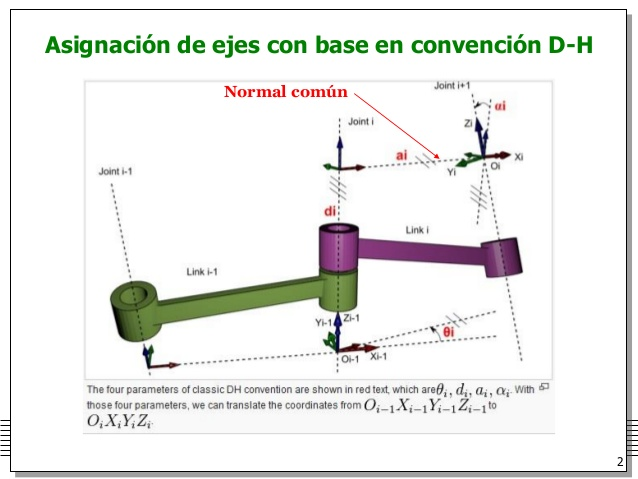
\includegraphics[scale=0.6]{imagenes/grafica.jpg} imagen 1.2 
\begin{center}
\end{center}
\end{center}
\begin{center}
\large \huge Una convención comúnmente utilizada para seleccionar marcos de referencia en aplicaciones de robótica es la convención de Denavit y Hartenberg (D – H) que fue presentada por Jacques Denavit y Richard S. Hartenberg . En esta convención, los marcos de coordenadas se unen a las uniones entre dos enlaces de manera que una transformación se asocia con la unión, [Z], y la segunda se asocia con el enlace [X]. Las transformaciones de coordenadas a lo largo de un robot en serie que consta de n enlaces forman las ecuaciones cinemáticas del robot, en la imagen 1.3 se muestra la formula de la matriz
\end{center}

\begin{center}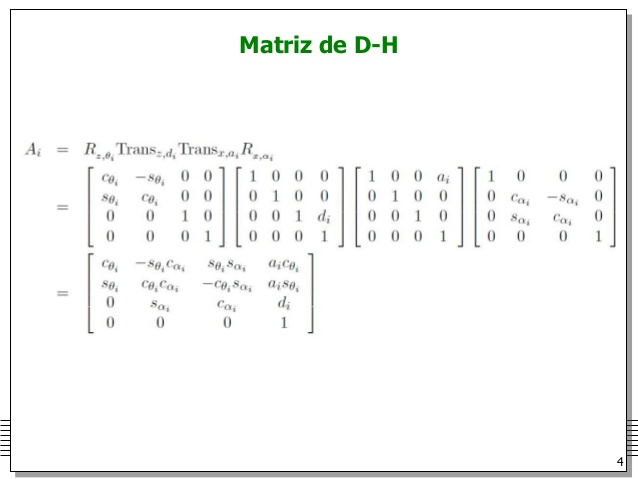
\includegraphics[scale=0.6]{imagenes/matriz.jpg}\\imagen 1.3
\end{center}
\begin{center}
\large \huge
 {Para determinar las transformaciones de coordenadas [Z] y [X], las juntas que conectan los enlaces se modelan como juntas articuladas o deslizantes, cada una de las cuales tiene una línea única S en el espacio que forma el eje de la junta y define el movimiento relativo de Los dos enlaces. Un robot en serie típico se caracteriza por una secuencia de seis líneas S i , i  = 1, ..., 6, una para cada articulación en el robot. Para cada secuencia de líneas S i y S i +1 , hay una línea normal común A i , i +1}\cite{santos2006reported}
\end{center}

\vspace{7cm}
 BIBLIOGRAFIA
\cite{santos2006reported}
\bibliographystyle{plain}
\bibliography{biblio}


\end{document}